\chapter{Detector Applications to measuring the active brain}

\section{{F}unctional {N}ear-{I}nfrared {fNIR} Imaging}
% detector applicaitons to improving fNIR
\begin{figure}[b]
  \begin{center}
    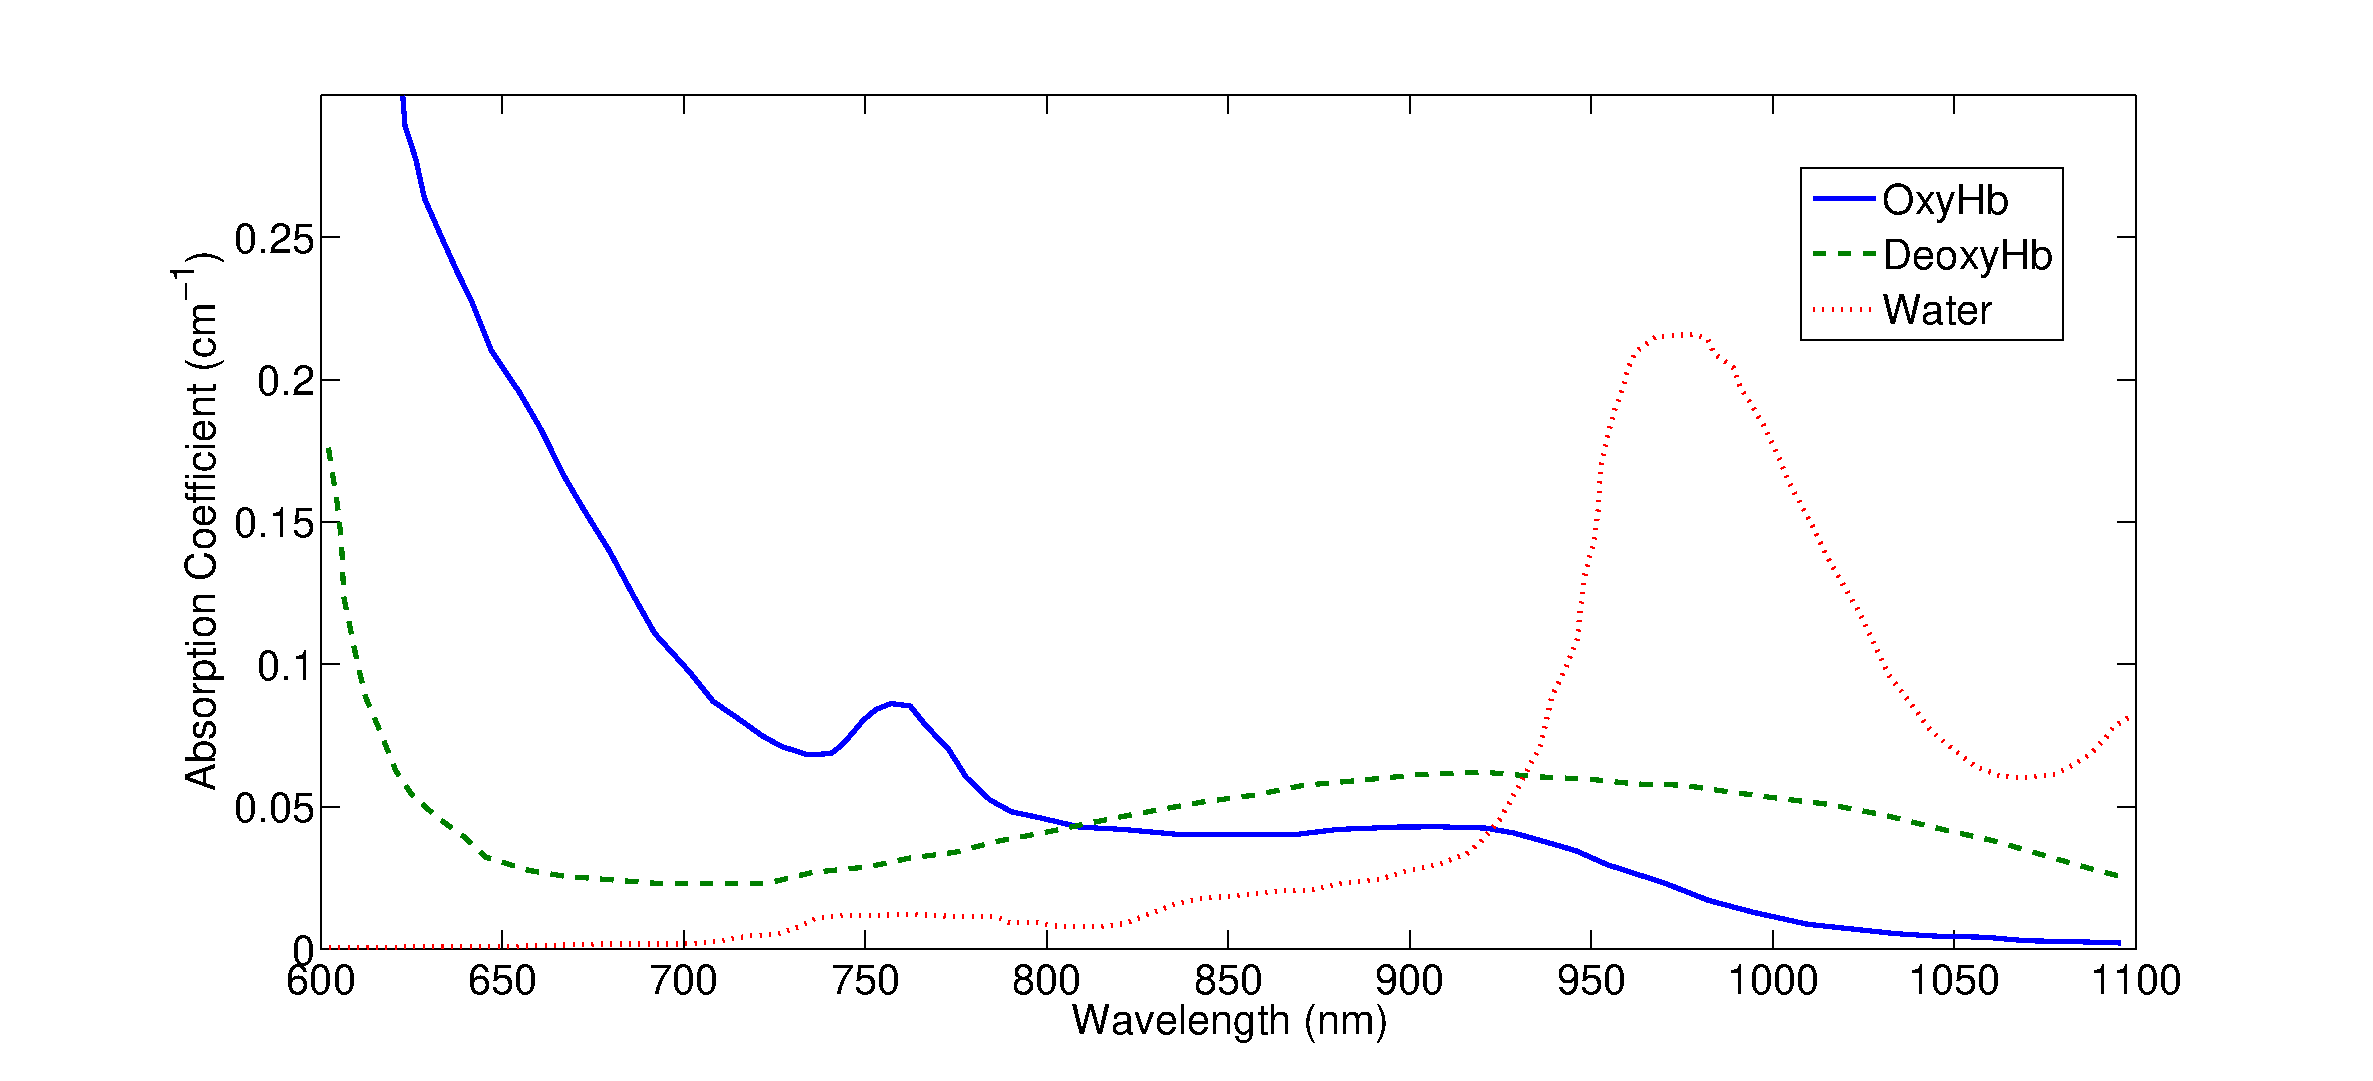
\includegraphics{AbsorptionData}
    \caption[Absorption spectra of water, deoxyhemoglobin and oxyhemoblogin]{\label{fig:fnirabsorption} Absorption spectra of water, Hb and Dhb.  From \citet{cope} and HB stuff from \citet{horecker} }
  \end{center}
\end{figure}

\begin{equation}
  I = I_0 e^{-\alpha x} \label{eq:beerlambert}
\end{equation}


\section{Temperature Measurements}
% Temperature imaging cameras.
% Limited to open skull because of low penetration depth.


From the Beer-Lambert law~\cref{eq:beerlambert}, the penetration depth, $\delta_{p}$ can be expressed as 
\begin{equation}
  \delta = \frac{1}{\alpha} \label{eq:penetrationdepth}
\end{equation}
where $\alpha$ is the absorption coefficient.  At body temperature (37\degree) the peak wavelength in the blackbody spectrum is approximately BLA.  For water at this wavelength, $\alpha$ is approximately HUGE, so $\delta$ is VERY SMALL. 